% 0L  
\vspace*{\fill}
\begin{figure}[h!]
    \centering
    \begin{subfigure}[b]{\textwidth}
        \centering
        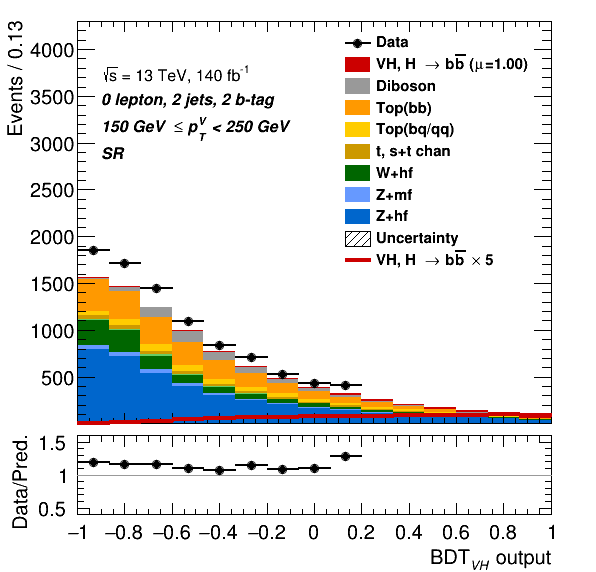
\includegraphics[width=0.32\textwidth]{Images/VH/Own_fit/prefit_VHbb/Region_distmva_BMax250_BMin150_DSR_J2_TTypebb_T2_L0_Y6051_Prefit.png}
        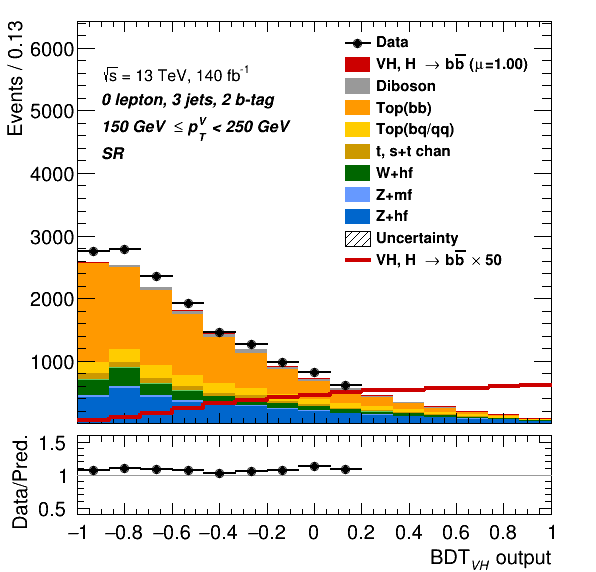
\includegraphics[width=0.32\textwidth]{Images/VH/Own_fit/prefit_VHbb/Region_distmva_BMax250_BMin150_DSR_J3_TTypebb_T2_L0_Y6051_Prefit.png}
        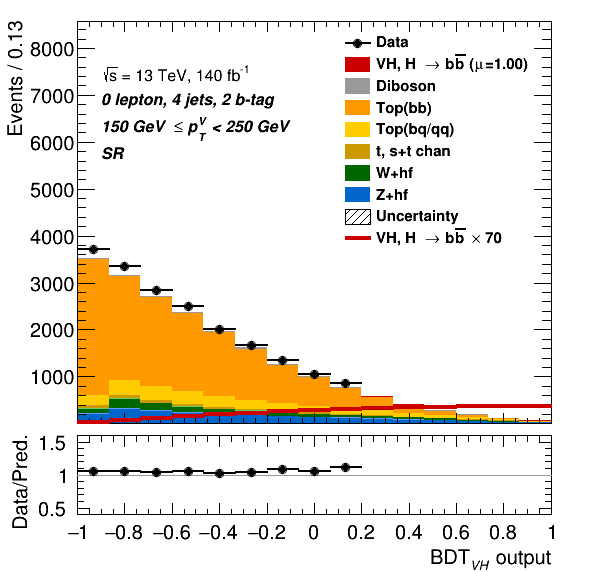
\includegraphics[width=0.32\textwidth]{Images/VH/Own_fit/prefit_VHbb/Region_distmva_BMax250_BMin150_DSR_J4_TTypebb_T2_L0_Y6051_Prefit.png}
        \caption{150 < \ptv\ < 250 GeV.}
        \label{fig:plots_VHbb_OL_150_SR}
    \end{subfigure}
    \begin{subfigure}[b]{\textwidth}
        \centering
        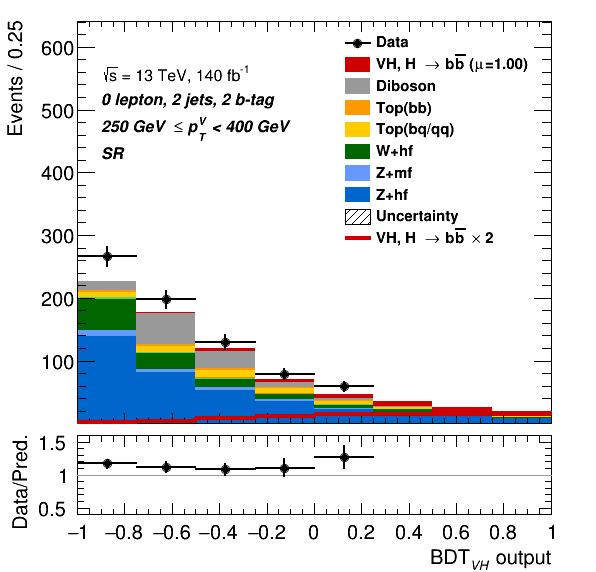
\includegraphics[width=0.32\textwidth]{Images/VH/Own_fit/prefit_VHbb/Region_distmva_BMax400_BMin250_DSR_J2_TTypebb_T2_L0_Y6051_Prefit.png}
        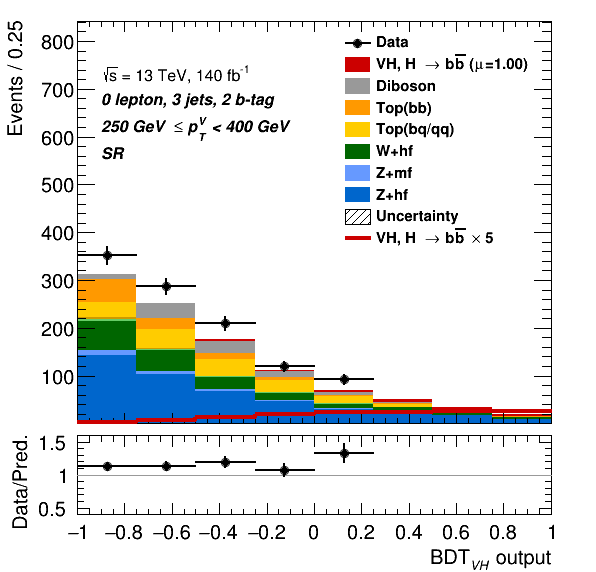
\includegraphics[width=0.32\textwidth]{Images/VH/Own_fit/prefit_VHbb/Region_distmva_BMax400_BMin250_DSR_J3_TTypebb_T2_L0_Y6051_Prefit.png}
        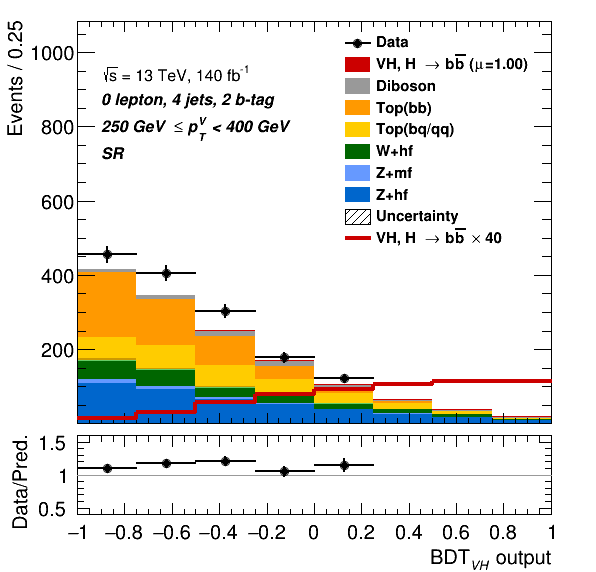
\includegraphics[width=0.32\textwidth]{Images/VH/Own_fit/prefit_VHbb/Region_distmva_BMax400_BMin250_DSR_J4_TTypebb_T2_L0_Y6051_Prefit.png}
        \caption{250 < \ptv\ < 400 GeV.}
        \label{fig:plots_VHbb_OL_250_SR}
    \end{subfigure}
    \caption{The 0L signal regions in the $BB$-tagged 2-jet (left), 3-jet (centre), and 4-jet (right).}
    \label{fig:plots_VHbb_OL_SR}
\end{figure} 

\begin{figure}[h!]
    \centering
    \begin{subfigure}[b]{\textwidth}
        \centering
        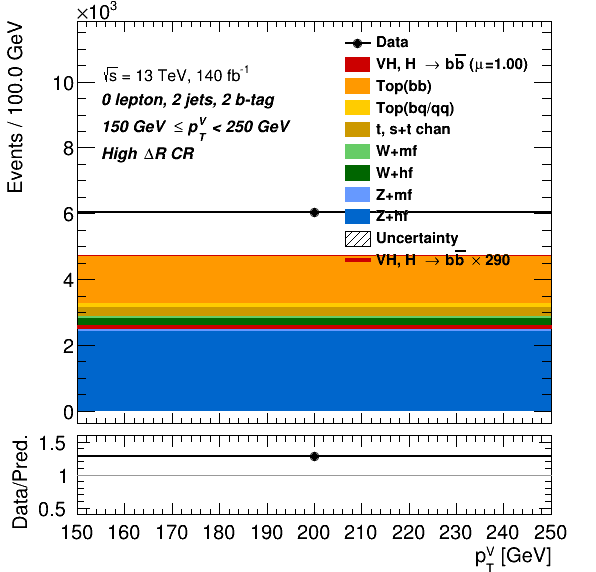
\includegraphics[width=0.32\textwidth]{Images/VH/Own_fit/prefit_VHbb/Region_distpTV_BMax250_BMin150_DCRHigh_J2_TTypebb_T2_L0_Y6051_Prefit.png}
        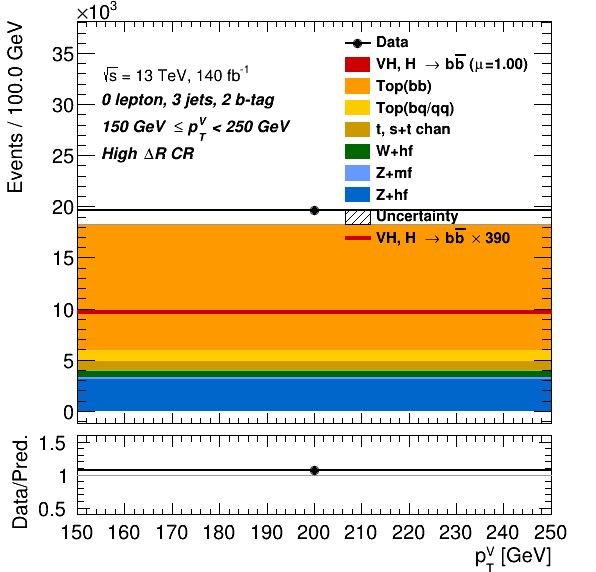
\includegraphics[width=0.32\textwidth]{Images/VH/Own_fit/prefit_VHbb/Region_distpTV_BMax250_BMin150_DCRHigh_J3_TTypebb_T2_L0_Y6051_Prefit.png}
        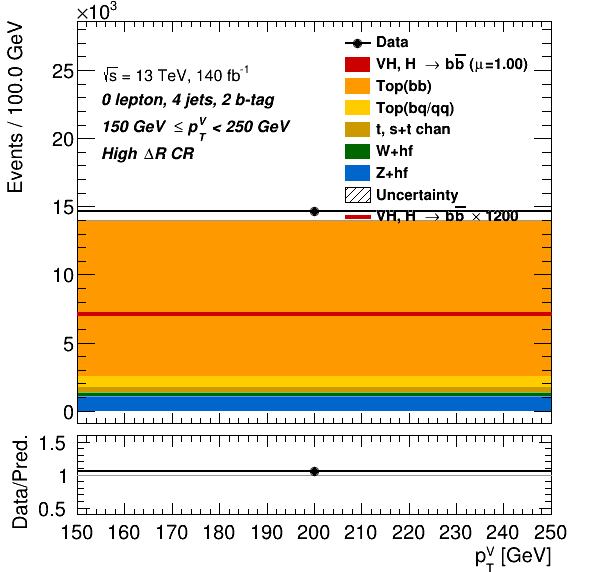
\includegraphics[width=0.32\textwidth]{Images/VH/Own_fit/prefit_VHbb/Region_distpTV_BMax250_BMin150_DCRHigh_J4_TTypebb_T2_L0_Y6051_Prefit.png}
        \caption{150 < \ptv\ < 250 GeV.}
        \label{fig:plots_VHbb_OL_150_CRH}
    \end{subfigure}
    \begin{subfigure}[b]{\textwidth}
        \centering
        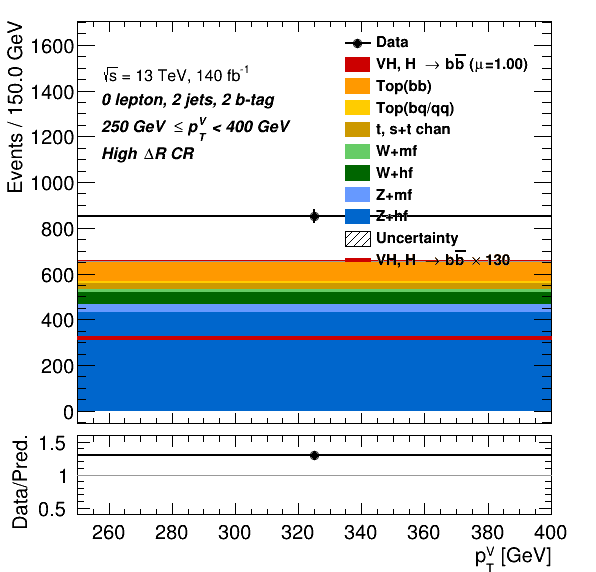
\includegraphics[width=0.32\textwidth]{Images/VH/Own_fit/prefit_VHbb/Region_distpTV_BMax400_BMin250_DCRHigh_J2_TTypebb_T2_L0_Y6051_Prefit.png}
        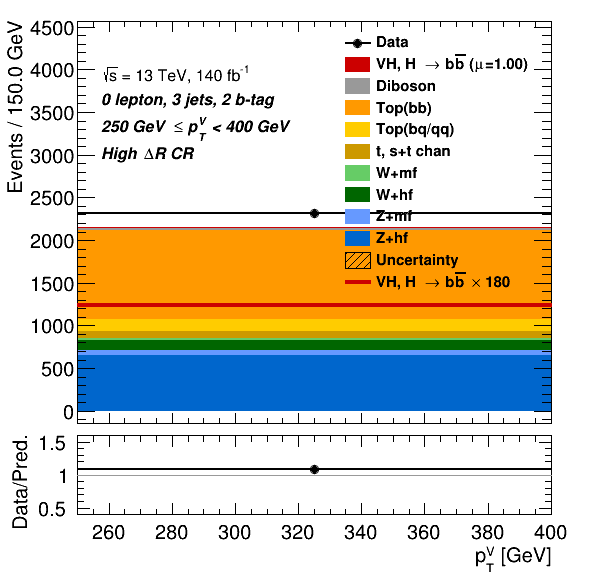
\includegraphics[width=0.32\textwidth]{Images/VH/Own_fit/prefit_VHbb/Region_distpTV_BMax400_BMin250_DCRHigh_J3_TTypebb_T2_L0_Y6051_Prefit.png}
        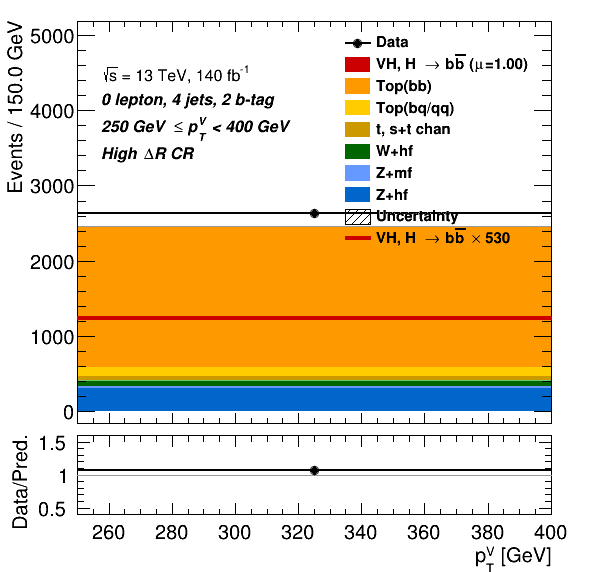
\includegraphics[width=0.32\textwidth]{Images/VH/Own_fit/prefit_VHbb/Region_distpTV_BMax400_BMin250_DCRHigh_J4_TTypebb_T2_L0_Y6051_Prefit.png}
        \caption{250 < \ptv\ < 400 GeV.}
        \label{fig:plots_VHbb_OL_250_CRH}
    \end{subfigure}
    \caption{The 0L \highdr\ CR in the $BB$-tagged 2-jet (left), 3-jet (centre), and 4-jet (right).}
    \label{fig:plots_VHbb_OL_CRH}
\end{figure} 

\vspace*{\fill} 

% 1L
\begin{figure}[h!]
    \centering
    \begin{subfigure}[b]{\textwidth}
        \centering
        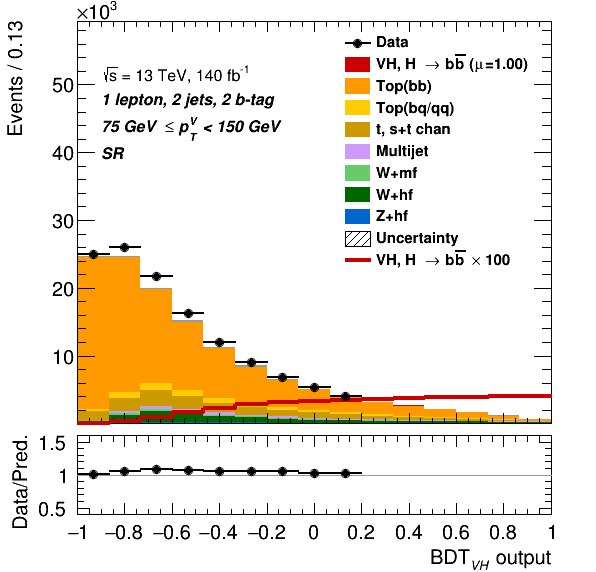
\includegraphics[width=0.40\textwidth]{Images/VH/Own_fit/prefit_VHbb/Region_distmva_BMax150_BMin75_DSR_J2_TTypebb_T2_L1_Y6051_Prefit.png}
        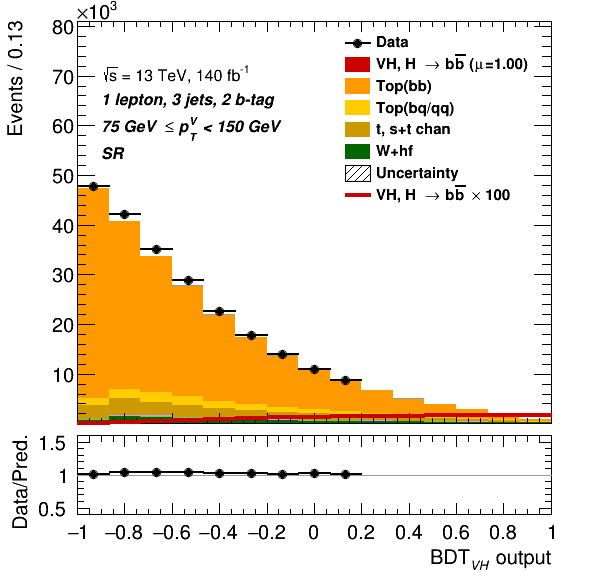
\includegraphics[width=0.40\textwidth]{Images/VH/Own_fit/prefit_VHbb/Region_distmva_BMax150_BMin75_DSR_J3_TTypebb_T2_L1_Y6051_Prefit.png}
        \caption{75 < \ptv\ < 150 GeV.}
        \label{fig:plots_VHbb_1L_75_SR}
    \end{subfigure}
    \begin{subfigure}[b]{\textwidth}
        \centering
        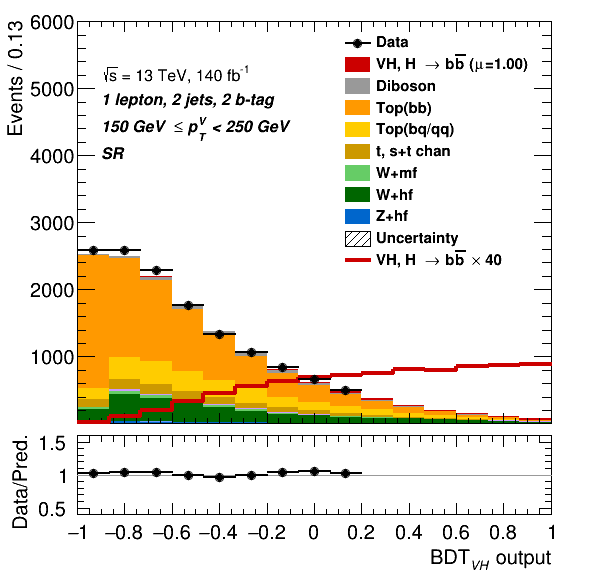
\includegraphics[width=0.40\textwidth]{Images/VH/Own_fit/prefit_VHbb/Region_distmva_BMax250_BMin150_DSR_J2_TTypebb_T2_L1_Y6051_Prefit.png}
        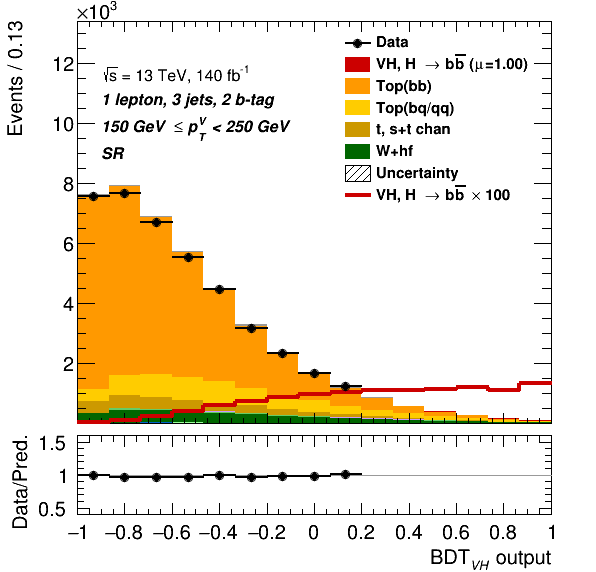
\includegraphics[width=0.40\textwidth]{Images/VH/Own_fit/prefit_VHbb/Region_distmva_BMax250_BMin150_DSR_J3_TTypebb_T2_L1_Y6051_Prefit.png}
        \caption{150 < \ptv\ < 250 GeV.}
        \label{fig:plots_VHbb_1L_150_SR}
    \end{subfigure}
    \begin{subfigure}[b]{\textwidth}
        \centering
        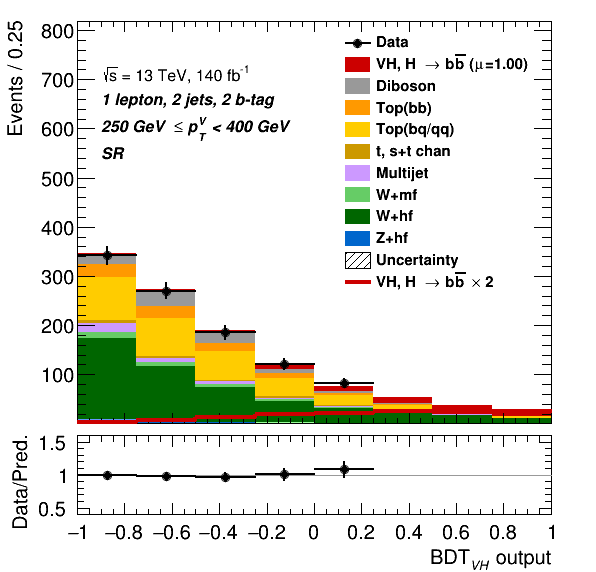
\includegraphics[width=0.40\textwidth]{Images/VH/Own_fit/prefit_VHbb/Region_distmva_BMax400_BMin250_DSR_J2_TTypebb_T2_L1_Y6051_Prefit.png}
        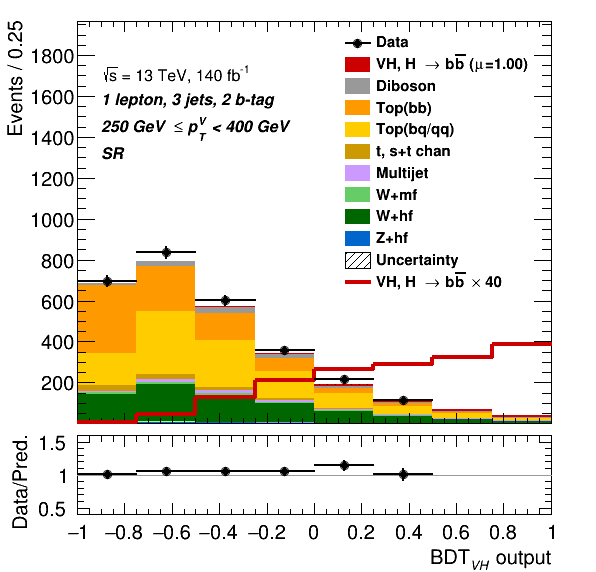
\includegraphics[width=0.40\textwidth]{Images/VH/Own_fit/prefit_VHbb/Region_distmva_BMax400_BMin250_DSR_J3_TTypebb_T2_L1_Y6051_Prefit.png}
        \caption{250 < \ptv\ < 400 GeV.}
        \label{fig:plots_VHbb_1L_250_SR}
    \end{subfigure}
    \caption{The 1L signal regions in the $BB$-tagged 2-jet (left) and 3-jet (right).}
    \label{fig:plots_VHbb_1L_SR}
\end{figure} 

\vspace*{\fill} \clearpage
\vspace*{\fill}

\begin{figure}[h!]
    \centering
    \begin{subfigure}[b]{\textwidth}
        \centering
        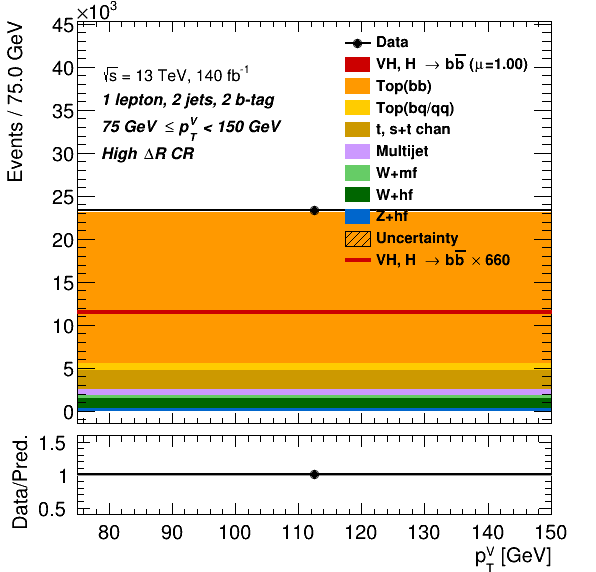
\includegraphics[width=0.40\textwidth]{Images/VH/Own_fit/prefit_VHbb/Region_distpTV_BMax150_BMin75_DCRHigh_J2_TTypebb_T2_L1_Y6051_Prefit.png}
        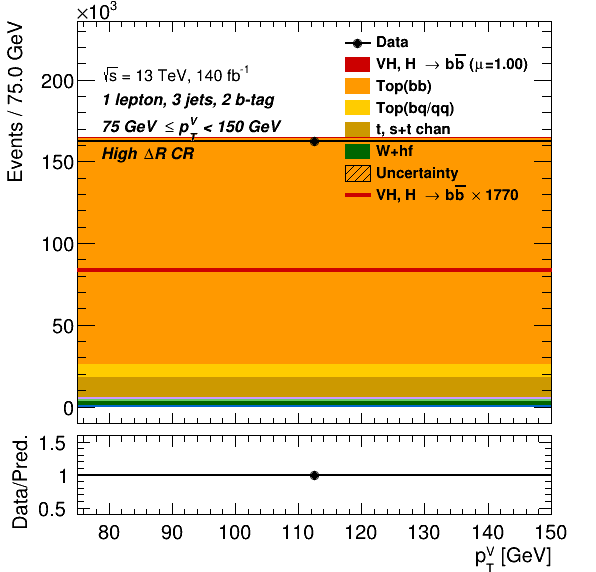
\includegraphics[width=0.40\textwidth]{Images/VH/Own_fit/prefit_VHbb/Region_distpTV_BMax150_BMin75_DCRHigh_J3_TTypebb_T2_L1_Y6051_Prefit.png}
        \caption{75 < \ptv\ < 150 GeV.}
        \label{fig:plots_VHbb_1L_75_CRH}
    \end{subfigure}
    \begin{subfigure}[b]{\textwidth}
        \centering
        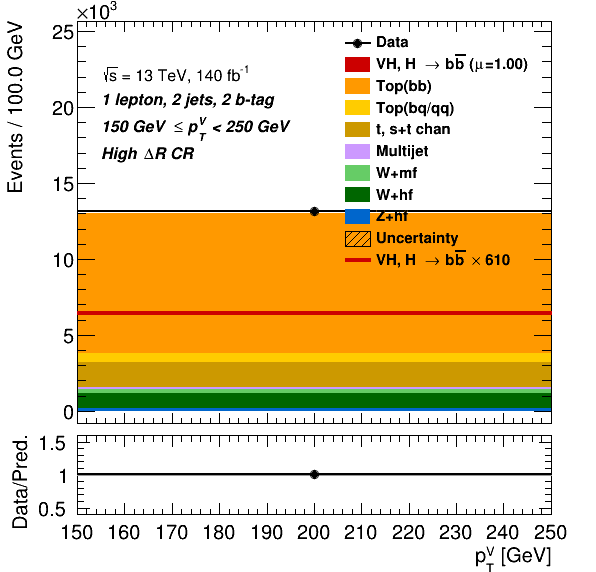
\includegraphics[width=0.40\textwidth]{Images/VH/Own_fit/prefit_VHbb/Region_distpTV_BMax250_BMin150_DCRHigh_J2_TTypebb_T2_L1_Y6051_Prefit.png}
        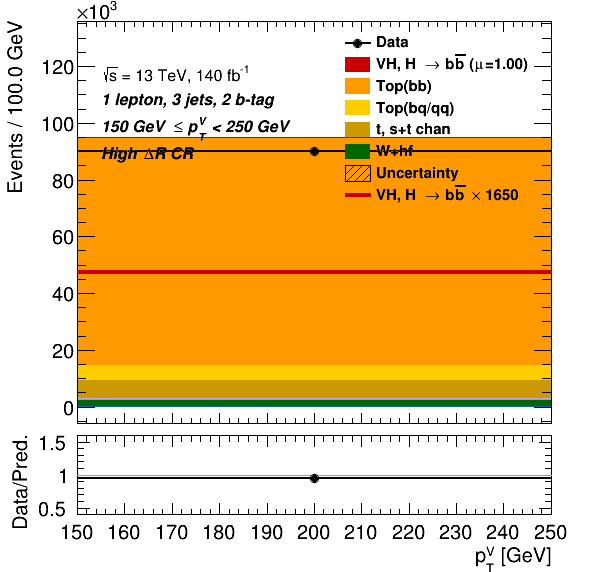
\includegraphics[width=0.40\textwidth]{Images/VH/Own_fit/prefit_VHbb/Region_distpTV_BMax250_BMin150_DCRHigh_J3_TTypebb_T2_L1_Y6051_Prefit.png}
        \caption{150 < \ptv\ < 250 GeV.}
        \label{fig:plots_VHbb_1L_150_CRH}
    \end{subfigure}
    \begin{subfigure}[b]{\textwidth}
        \centering
        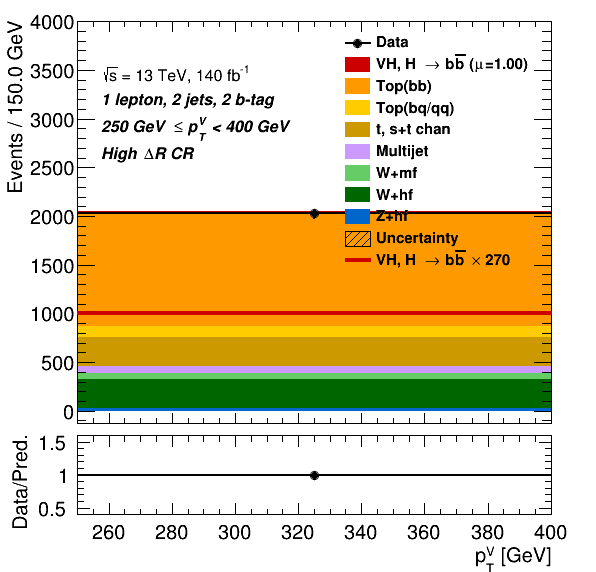
\includegraphics[width=0.40\textwidth]{Images/VH/Own_fit/prefit_VHbb/Region_distpTV_BMax400_BMin250_DCRHigh_J2_TTypebb_T2_L1_Y6051_Prefit.png}
        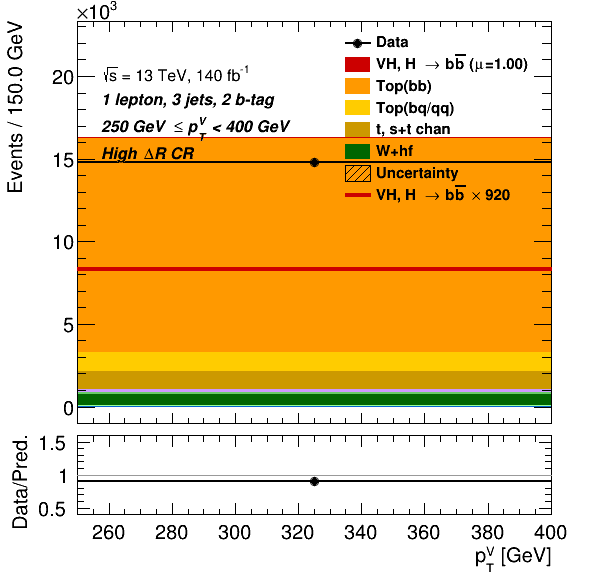
\includegraphics[width=0.40\textwidth]{Images/VH/Own_fit/prefit_VHbb/Region_distpTV_BMax400_BMin250_DCRHigh_J3_TTypebb_T2_L1_Y6051_Prefit.png}
        \caption{250 < \ptv\ < 400 GeV.}
        \label{fig:plots_VHbb_1L_250_CRH}
    \end{subfigure}
    \caption{The 1L \highdr\ CR in the $BB$-tagged 2-jet (left) and 3-jet (right).}
    \label{fig:plots_VHbb_1L_CRH}
\end{figure} 

\vspace*{\fill} \clearpage
\vspace*{\fill}


\begin{figure}[h!]
    \centering
    \begin{subfigure}[b]{\textwidth}
        \centering
        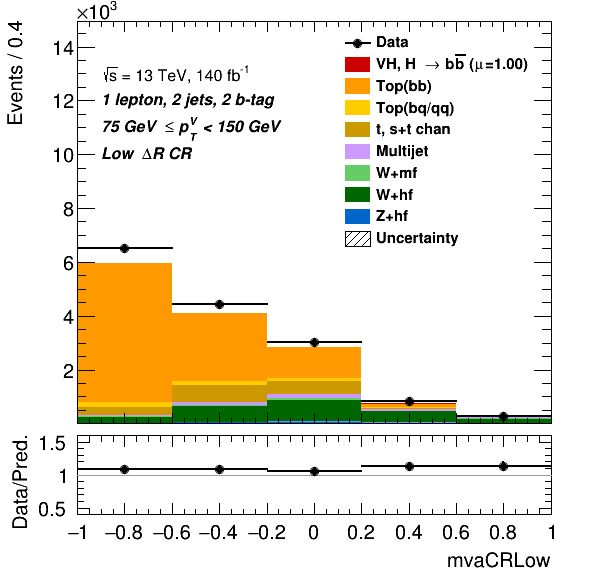
\includegraphics[width=0.40\textwidth]{Images/VH/Own_fit/prefit_VHbb/Region_distmvaCRLow_BMax150_BMin75_DCRLow_J2_TTypebb_T2_L1_Y6051_Prefit.png}
        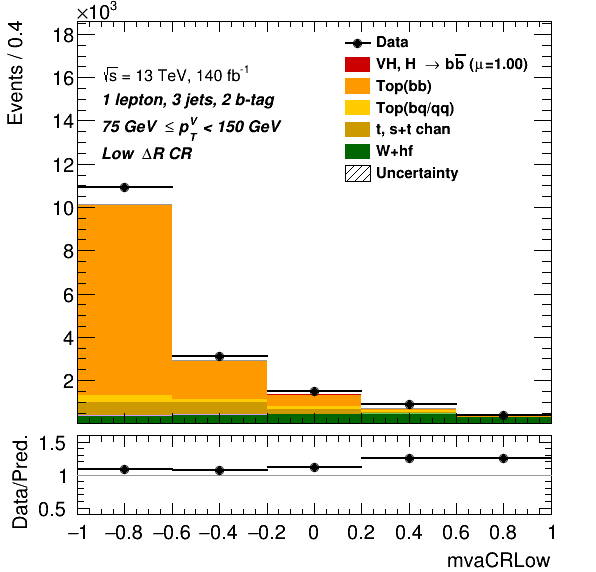
\includegraphics[width=0.40\textwidth]{Images/VH/Own_fit/prefit_VHbb/Region_distmvaCRLow_BMax150_BMin75_DCRLow_J3_TTypebb_T2_L1_Y6051_Prefit.png}
        \caption{75 < \ptv\ < 150 GeV.}
        \label{fig:plots_VHbb_1L_75_CRL}
    \end{subfigure}
    \begin{subfigure}[b]{\textwidth}
        \centering
        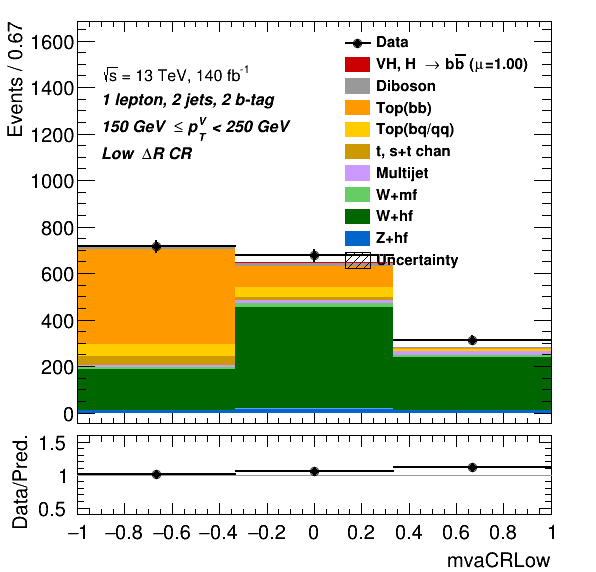
\includegraphics[width=0.40\textwidth]{Images/VH/Own_fit/prefit_VHbb/Region_distmvaCRLow_BMax250_BMin150_DCRLow_J2_TTypebb_T2_L1_Y6051_Prefit.png}
        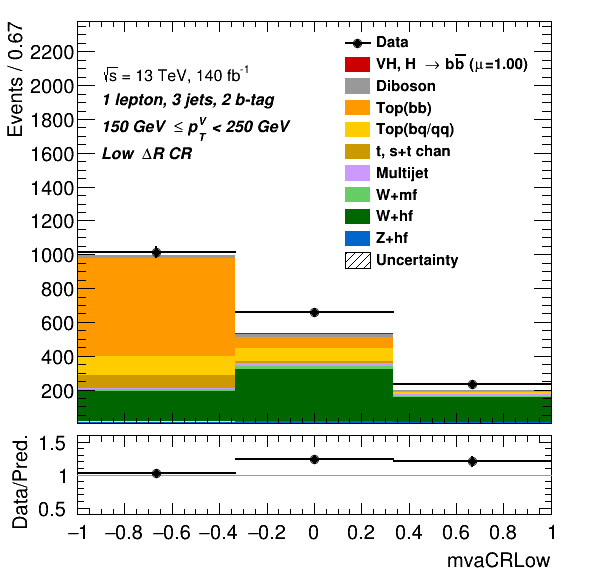
\includegraphics[width=0.40\textwidth]{Images/VH/Own_fit/prefit_VHbb/Region_distmvaCRLow_BMax250_BMin150_DCRLow_J3_TTypebb_T2_L1_Y6051_Prefit.png}
        \caption{150 < \ptv\ < 250 GeV.}
        \label{fig:plots_VHbb_1L_150_CRL}
    \end{subfigure}
    \begin{subfigure}[b]{\textwidth}
        \centering
        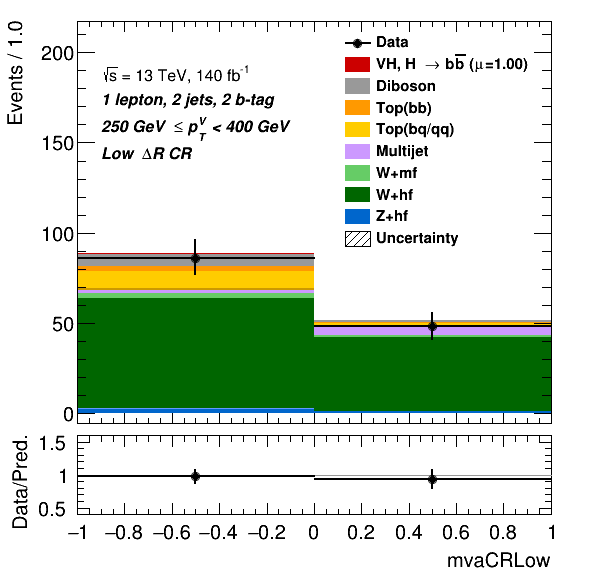
\includegraphics[width=0.40\textwidth]{Images/VH/Own_fit/prefit_VHbb/Region_distmvaCRLow_BMax400_BMin250_DCRLow_J2_TTypebb_T2_L1_Y6051_Prefit.png}
        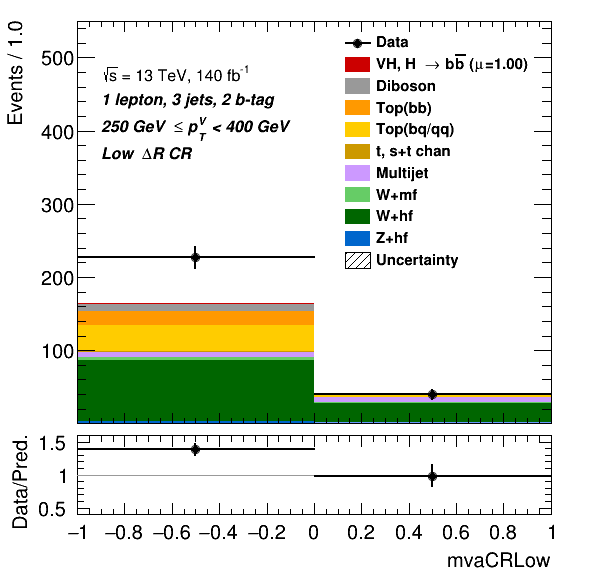
\includegraphics[width=0.40\textwidth]{Images/VH/Own_fit/prefit_VHbb/Region_distmvaCRLow_BMax400_BMin250_DCRLow_J3_TTypebb_T2_L1_Y6051_Prefit.png}
        \caption{250 < \ptv\ < 400 GeV.}
        \label{fig:plots_VHbb_1L_250_CRL}
    \end{subfigure}
    \caption{The 1L \lowdr\ CR in the $BB$-tagged.}
    \label{fig:plots_VHbb_1L_CRL}
\end{figure} 

\vspace*{\fill} \clearpage
\vspace*{\fill}

% 2L
\begin{figure}[h!]
    \centering
    \begin{subfigure}[b]{\textwidth}
        \centering
        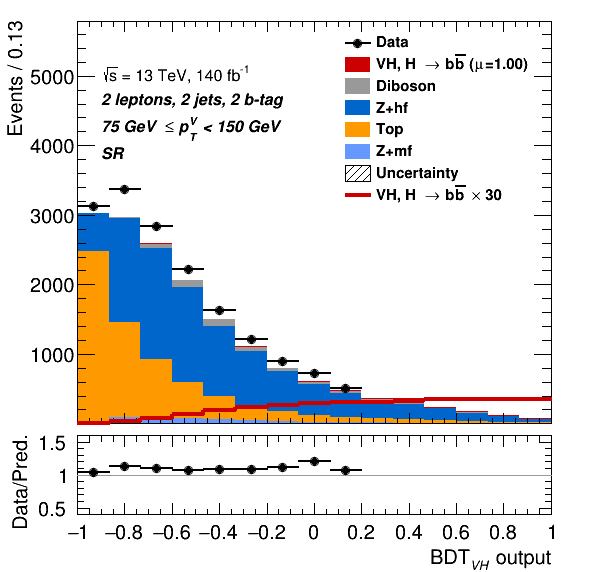
\includegraphics[width=0.32\textwidth]{Images/VH/Own_fit/prefit_VHbb/Region_distmva_BMax150_BMin75_DSR_J2_TTypebb_T2_L2_Y6051_Prefit.png}
        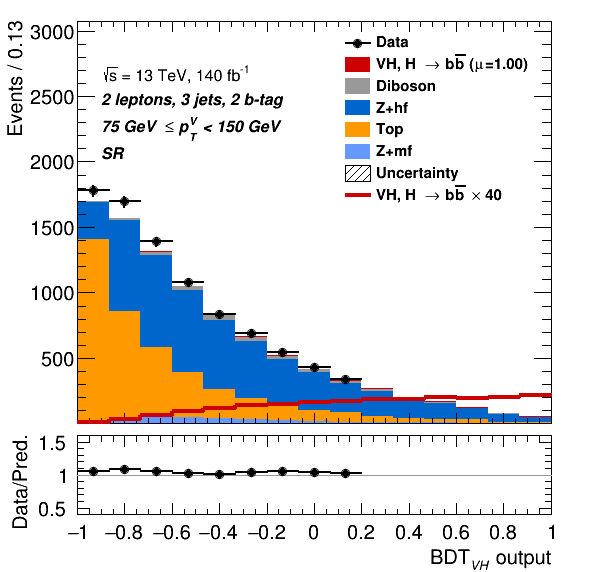
\includegraphics[width=0.32\textwidth]{Images/VH/Own_fit/prefit_VHbb/Region_distmva_BMax150_BMin75_DSR_J3_TTypebb_T2_L2_Y6051_Prefit.png}
        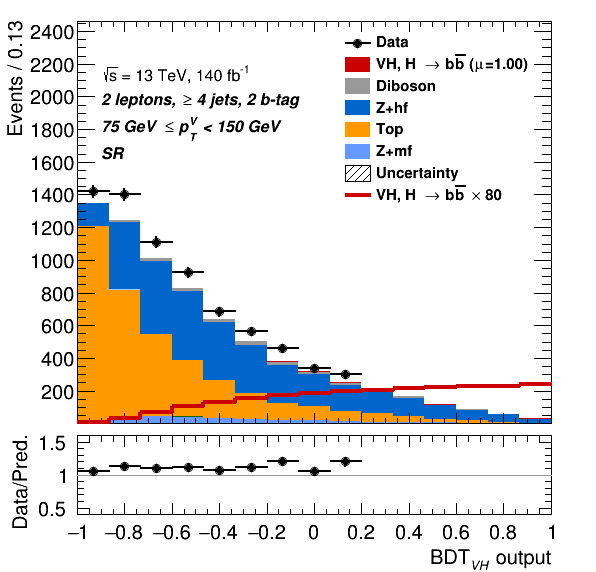
\includegraphics[width=0.32\textwidth]{Images/VH/Own_fit/prefit_VHbb/Region_distmva_BMax150_BMin75_DSR_J4_TTypebb_incJet1_T2_L2_Y6051_Prefit.png}
        \caption{75 < \ptv\ < 150 GeV.}
        \label{fig:plots_VHbb_2L_75_SR}
    \end{subfigure}
    \begin{subfigure}[b]{\textwidth}
        \centering
        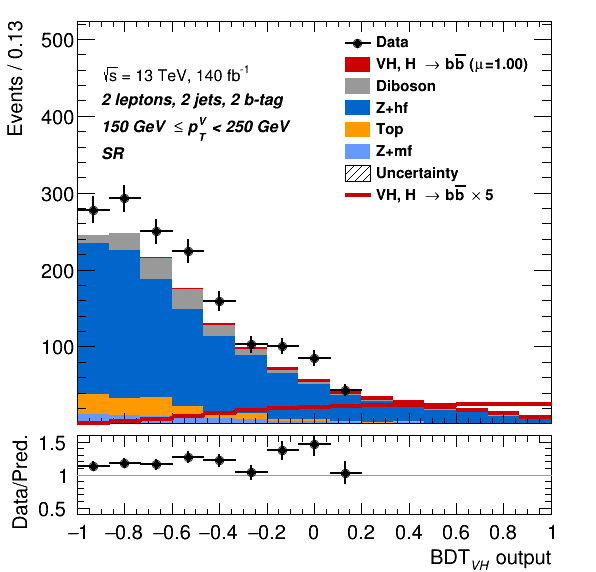
\includegraphics[width=0.32\textwidth]{Images/VH/Own_fit/prefit_VHbb/Region_distmva_BMax250_BMin150_DSR_J2_TTypebb_T2_L2_Y6051_Prefit.png}
        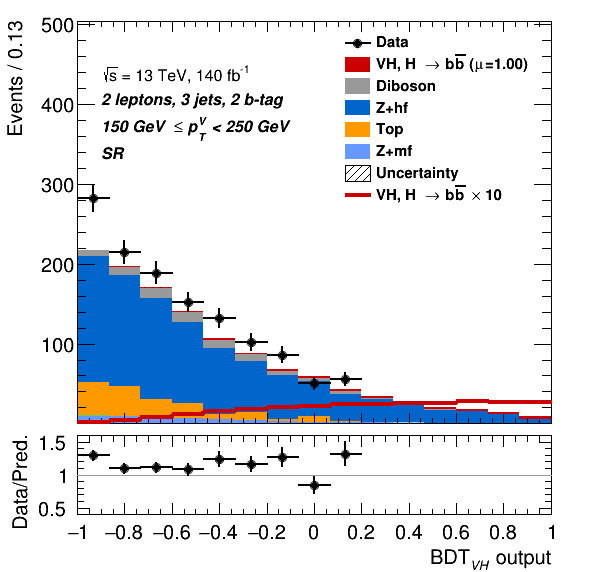
\includegraphics[width=0.32\textwidth]{Images/VH/Own_fit/prefit_VHbb/Region_distmva_BMax250_BMin150_DSR_J3_TTypebb_T2_L2_Y6051_Prefit.png}
        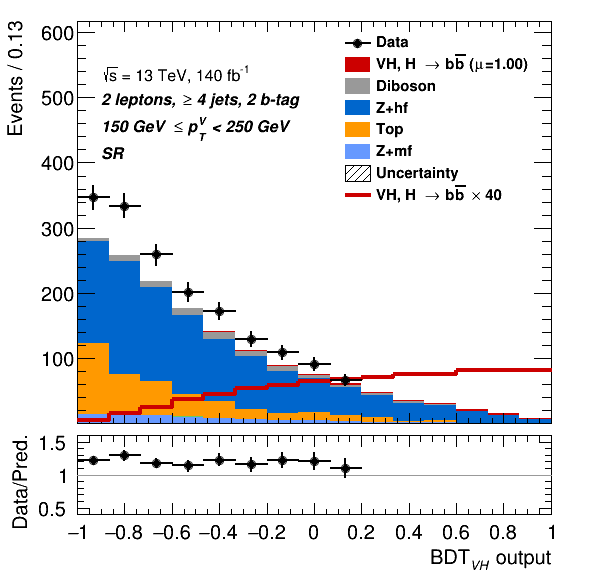
\includegraphics[width=0.32\textwidth]{Images/VH/Own_fit/prefit_VHbb/Region_distmva_BMax250_BMin150_DSR_J4_TTypebb_incJet1_T2_L2_Y6051_Prefit.png}
        \caption{150 < \ptv\ < 250 GeV.}
        \label{fig:plots_VHbb_2L_150_SR}
    \end{subfigure}
    \begin{subfigure}[b]{\textwidth}
        \centering
        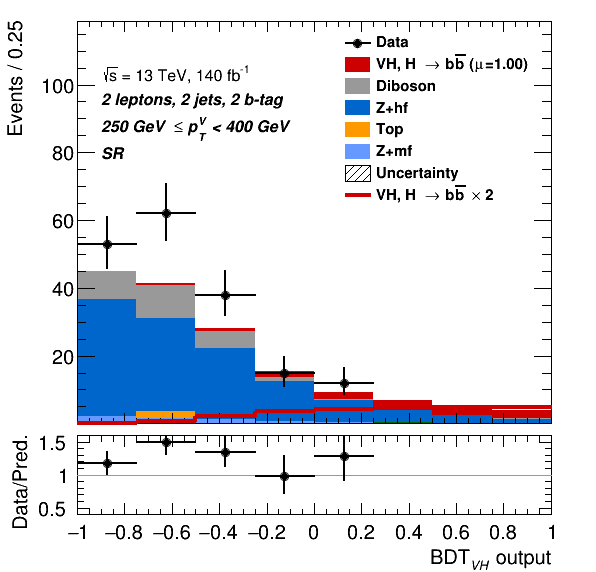
\includegraphics[width=0.32\textwidth]{Images/VH/Own_fit/prefit_VHbb/Region_distmva_BMax400_BMin250_DSR_J2_TTypebb_T2_L2_Y6051_Prefit.png}
        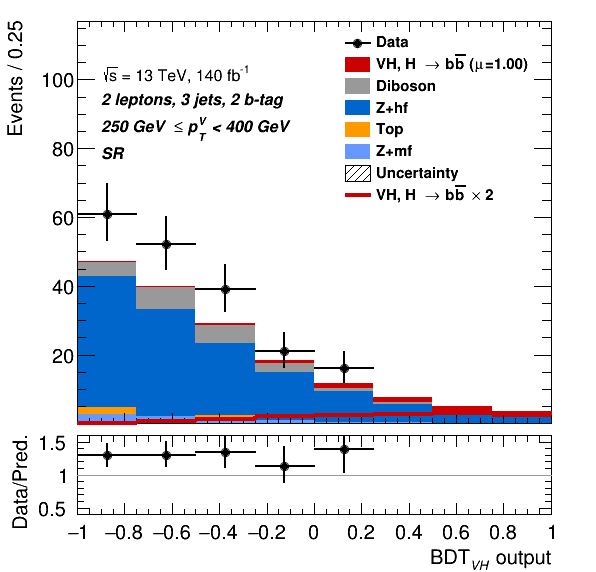
\includegraphics[width=0.32\textwidth]{Images/VH/Own_fit/prefit_VHbb/Region_distmva_BMax400_BMin250_DSR_J3_TTypebb_T2_L2_Y6051_Prefit.png}
        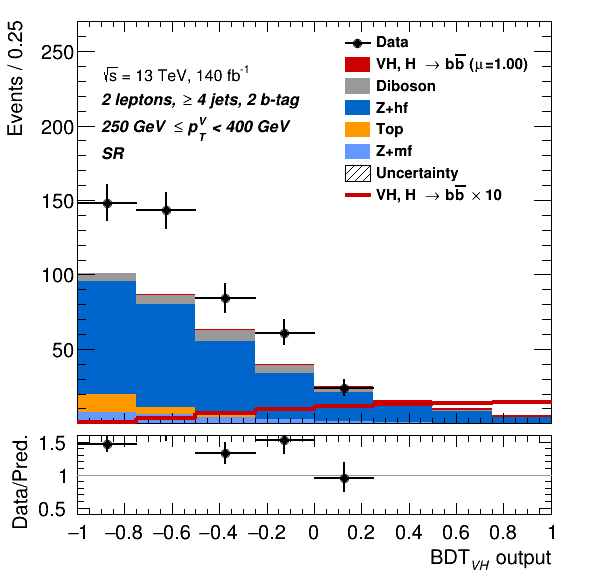
\includegraphics[width=0.32\textwidth]{Images/VH/Own_fit/prefit_VHbb/Region_distmva_BMax400_BMin250_DSR_J4_TTypebb_incJet1_T2_L2_Y6051_Prefit.png}
        \caption{250 < \ptv\ < 400 GeV.}
        \label{fig:plots_VHbb_2L_250_SR}
    \end{subfigure}
    \caption{The 2L signal regions in the $BB$-tagged 2-jet (left), 3-jet (centre), and $\geq$4-jet (right).}
     \label{fig:plots_VHbb_2L_SR}
\end{figure} 

\vspace*{\fill}\clearpage
\vspace*{\fill}

\begin{figure}[h!]
    \centering
    \begin{subfigure}[b]{\textwidth}
        \centering
        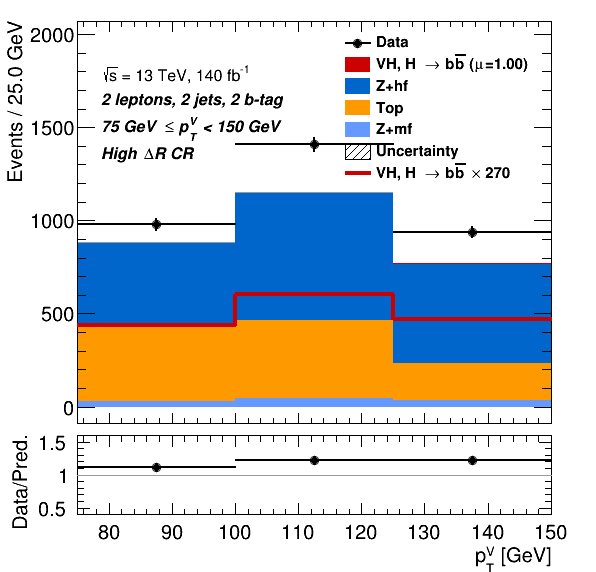
\includegraphics[width=0.32\textwidth]{Images/VH/Own_fit/prefit_VHbb/Region_distpTV_BMax150_BMin75_DCRHigh_J2_TTypebb_T2_L2_Y6051_Prefit.png}
        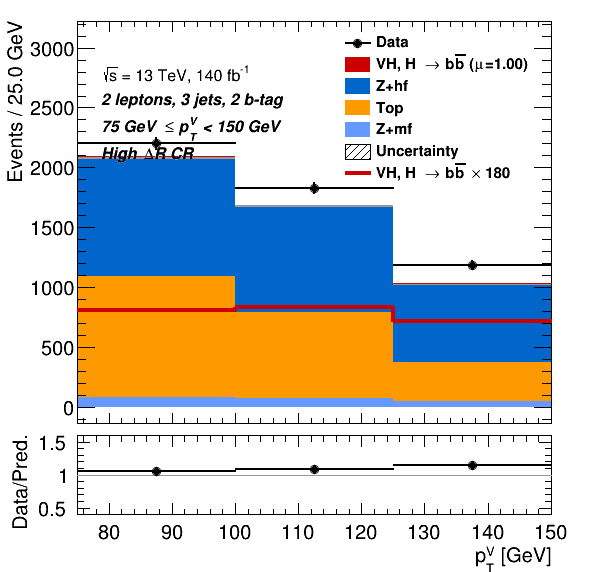
\includegraphics[width=0.32\textwidth]{Images/VH/Own_fit/prefit_VHbb/Region_distpTV_BMax150_BMin75_DCRHigh_J3_TTypebb_T2_L2_Y6051_Prefit.png}
        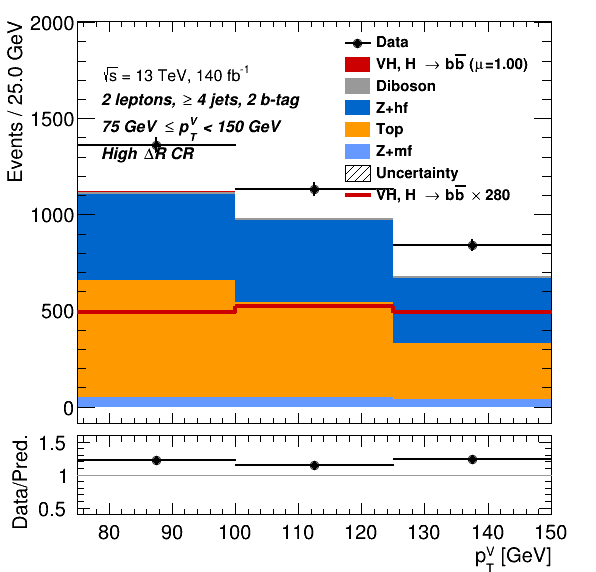
\includegraphics[width=0.32\textwidth]{Images/VH/Own_fit/prefit_VHbb/Region_distpTV_BMax150_BMin75_DCRHigh_J4_TTypebb_incJet1_T2_L2_Y6051_Prefit.png}
        \caption{75 < \ptv\ < 150 GeV.}
        \label{fig:plots_VHbb_2L_75_CRL}
    \end{subfigure}
    \begin{subfigure}[b]{\textwidth}
        \centering
        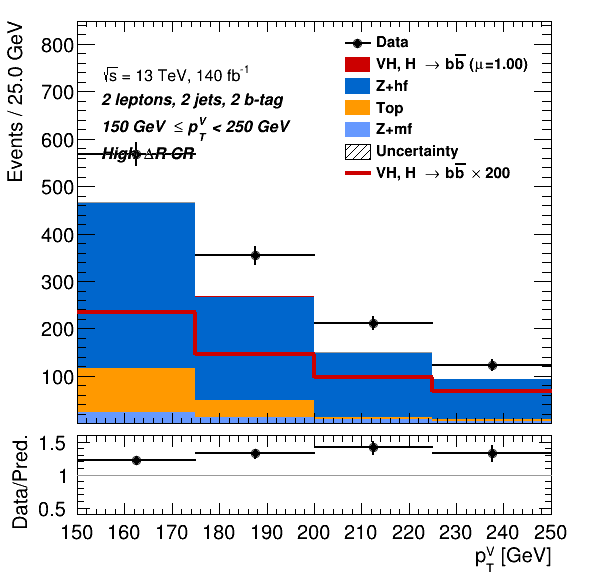
\includegraphics[width=0.32\textwidth]{Images/VH/Own_fit/prefit_VHbb/Region_distpTV_BMax250_BMin150_DCRHigh_J2_TTypebb_T2_L2_Y6051_Prefit.png}
        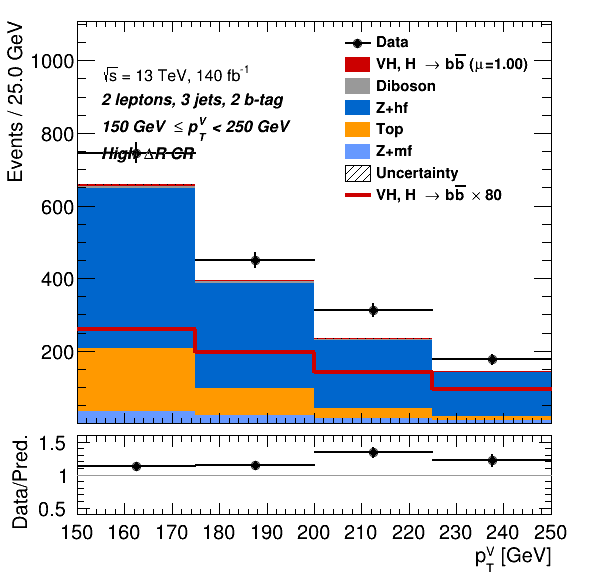
\includegraphics[width=0.32\textwidth]{Images/VH/Own_fit/prefit_VHbb/Region_distpTV_BMax250_BMin150_DCRHigh_J3_TTypebb_T2_L2_Y6051_Prefit.png}
        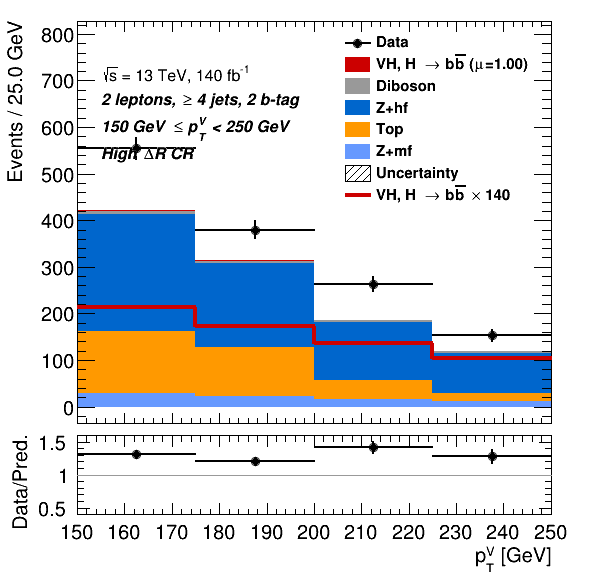
\includegraphics[width=0.32\textwidth]{Images/VH/Own_fit/prefit_VHbb/Region_distpTV_BMax250_BMin150_DCRHigh_J4_TTypebb_incJet1_T2_L2_Y6051_Prefit.png}
        \caption{150 < \ptv\ < 250 GeV.}
        \label{fig:plots_VHbb_2L_150_CRH}
    \end{subfigure}
    \begin{subfigure}[b]{\textwidth}
        \centering
        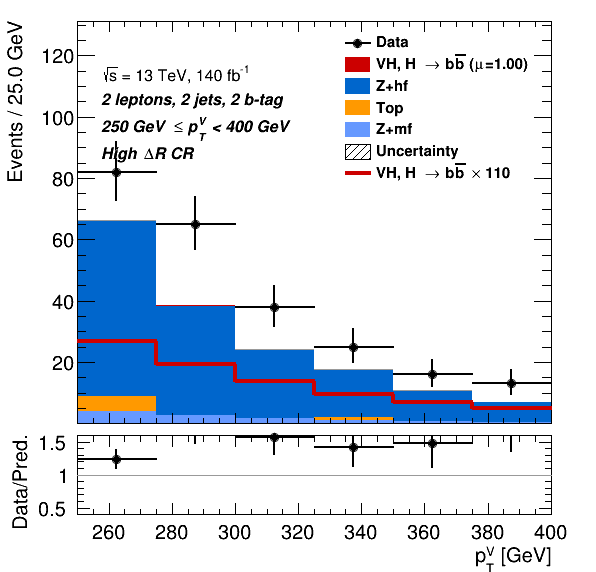
\includegraphics[width=0.32\textwidth]{Images/VH/Own_fit/prefit_VHbb/Region_distpTV_BMax400_BMin250_DCRHigh_J2_TTypebb_T2_L2_Y6051_Prefit.png}
        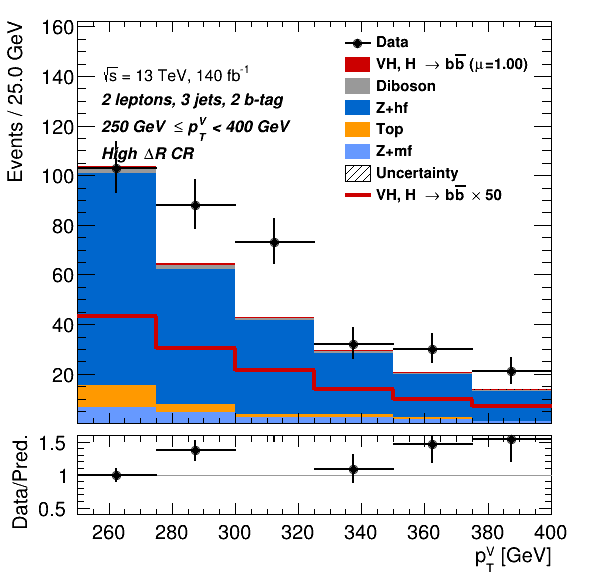
\includegraphics[width=0.32\textwidth]{Images/VH/Own_fit/prefit_VHbb/Region_distpTV_BMax400_BMin250_DCRHigh_J3_TTypebb_T2_L2_Y6051_Prefit.png}
        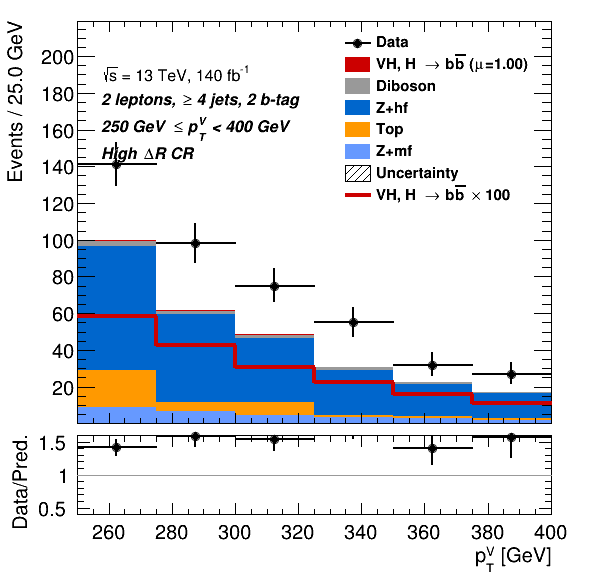
\includegraphics[width=0.32\textwidth]{Images/VH/Own_fit/prefit_VHbb/Region_distpTV_BMax400_BMin250_DCRHigh_J4_TTypebb_incJet1_T2_L2_Y6051_Prefit.png}
        \caption{250 < \ptv\ < 400 GeV.}
        \label{fig:plots_VHbb_2L_250_CRH}
    \end{subfigure}
    \caption{The 2L \highdr\ CR in the $BB$-tagged 2-jet (left), 3-jet (centre), and $\geq$4-jet (right).}
    \label{fig:plots_VHbb_2L_CRH}
\end{figure} 
\vspace*{\fill}